
\begin{figure}
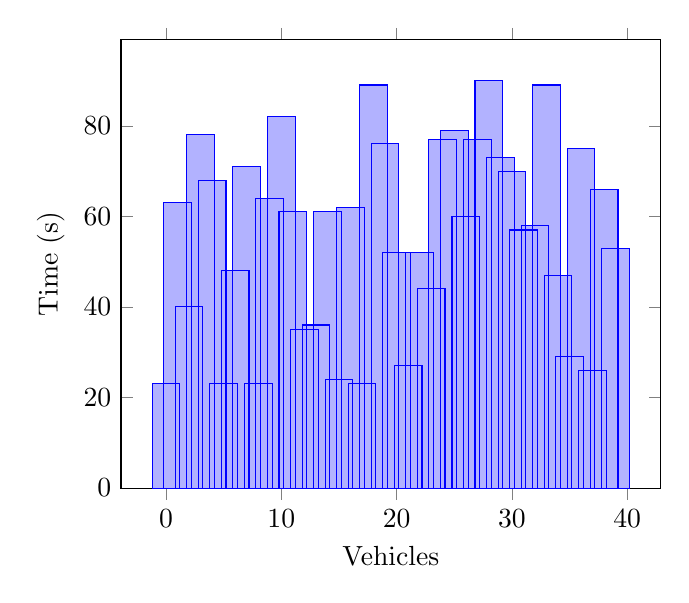
\begin{tikzpicture}
\begin{axis}[
legend style={anchor=west},
xlabel=Vehicles,
ylabel=Time (s),
ymin=0,
ybar,
]
\addplot coordinates {
(0, 23)
(1, 63)
(2, 40)
(3, 78)
(4, 68)
(5, 23)
(6, 48)
(7, 71)
(8, 23)
(9, 64)
(10, 82)
(11, 61)
(12, 35)
(13, 36)
(14, 61)
(15, 24)
(16, 62)
(17, 23)
(18, 89)
(19, 76)
(20, 52)
(21, 27)
(22, 52)
(23, 44)
(24, 77)
(25, 79)
(26, 60)
(27, 77)
(28, 90)
(29, 73)
(30, 70)
(31, 57)
(32, 58)
(33, 89)
(34, 47)
(35, 29)
(36, 75)
(37, 26)
(38, 66)
(39, 53)
};

\end{axis}
\end{tikzpicture}
\label{tik:100:2_O, 2_O.-60, 3_O}
\caption{100 percent diving with GSC on route $2_O, 2_O.-60, 3_O$}
\end{figure}
